
\documentclass{article}
    \usepackage[utf8]{inputenc}
    \usepackage{comment}
    \usepackage{environ}
    \usepackage{listings}
    \usepackage{xcolor}
    \usepackage[letterpaper, portrait, margin=1in]{geometry}
    \usepackage{amsmath}
    \usepackage{amssymb}
    \usepackage{graphicx}
    
    \newif\ifshowsolutions
    
    % comment the following line to hide solutions
    \showsolutionstrue
    
    \ifshowsolutions
        \newenvironment{solution}{

            \color{blue} \smallskip \textbf{Solution:}}{}
    \else
        \NewEnviron{solution} {
            \ \\
            \ \\
            \ \\
        }
    \fi
    
    \begin{document}
    
    \part*{Random Variables, Distributions, Indicators}
    \vspace{-7pt}
    \hrule
    \vspace{7pt}
    \section{Intro}
    \begin{enumerate}
        \item What is the definition of a random variable?
        \begin{solution}
            A random variable defined on a probability space $\Omega$ is a function $X \colon \Omega \rightarrow \mathbb{R}$. That is all it is!
            Often a random variable is defined on a probability space that corresponds exactly to the values it has. What I mean is that the events of
            $\Omega$ can be something like $A_0, A_1, \ldots, A_k, \ldots$ where $P(X = k) = P(A_k)$. This is how we define all the distributions.
        \end{solution}
        \item If $X$ is a random variable, what does $f(X)$ mean?
        \begin{solution}
            $f(X)$ is a new random variable on $\Omega$, such that $(f(X))(\omega) = f(X(\omega))$.
        \end{solution}
        \item What is the definition of expectation and variance? Can you interpret these in terms of the distributions of random variables?
        \begin{solution}
            For random variables on a discrete space, \[
                E[X] = \sum_{\omega \in \Omega} X(\omega) P(\omega) = \sum_{k} k P(X = k) = \mu
            \]

            You can think of expectation as telling you where the `center' of the distribution is. Over the long term, taking repeated samples from the same
            random variable approximates the expectation (this is called the law of large numbers).

            In general, the variance is defined as \[
                E[(X - \mu)^2] = E[X^2] - \mu^2
            \]
            This measures how `wide' the distribution is. It is literally measuring the expected deviation from the mean, and we take the square so that it doesn't
            all cancel out. Try this by yourself, computing $E[X - \mu]$.
        \end{solution}
        \item Give an example of something (in real life) that has a:
        \begin{enumerate}
            \item bernoulli distribution
            \begin{solution}
                A coin flip. We have $\Omega = \{H, T\}$ uniform (meaning all the probabilities are the same), $X(H) = 1$, $X(T) = 0$.
            \end{solution}
            \item binomial distribution
            \begin{solution}
                Multiple coin flips in a row! We have something like \[
                    \Omega = \{HHH, HHT, HTH, THH, HTT, THT, TTH, TTT\}
                \]
                With probabilities $1/8$ each. However, our $X$ ``summarizes'' and loses information! Let $X$ be the number of heads, Our X is defined as \[
                    X(HHH) = 3, X(HHT) = 2, X(HTH) = 2, X(THH) = 2, X(HTT) = 1, X(THT) = 1, X(TTH) = 1, X(TTT) = 0
                \]
                Then \[
                    P(X = 3) = 1/8, P(X = 2) = 3/8, P(X = 1) = 3/8, P(X = 0) = 1/8
                \]
                Which is binomial with $p = 1/2$ and $n = 3$.
            \end{solution}
            \item geometric distribution
            \begin{solution}
                You're trying to add a class on Cal Central. You hit enroll, let's say the chance of it actually enrolling you is $1/4$ each time. Then the geometric
                distribution models how many times you have to click the enroll button to actually be enrolled in the class.
                The probability of us being enrolled after 0 clicks is 0. After 1 click, it just has to work once, so $1/4$. After 2 clicks, it has to fail the first time and
                succeed the next, so $3/4 \cdot 1/4$. In general, \[
                    P(X = k) = \left(\frac{3}{4}\right)^{(k-1)} \frac{1}{4}
                \]
            \end{solution}
            \item poisson distribution
            \begin{solution}
                Berkeley has like 40,000 students. That's close enough to infinity. They're all on campus and want to use AirBears, let's say the average student attempts to connect
                to AirBears once an hour. Then on average, we'll have $40,000$ students attempting to access AirBears every hour. We can use Poisson with $\lambda = 40000$ to model how
                many students connect in an hour-long period. Remember that $\lambda$ tells us the average.
                
                This is what the distribution looks like for $\lambda=5$:

                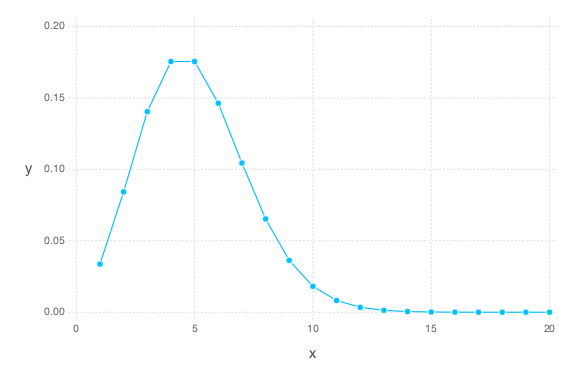
\includegraphics[height=4in,width=6in]{poisson_plot.png}

                I plotted it against several binomial distibutions, you can see how as $n \rightarrow \infty$ and $p \rightarrow 0$, but $np \rightarrow \lambda$ it converges to the Poisson:

                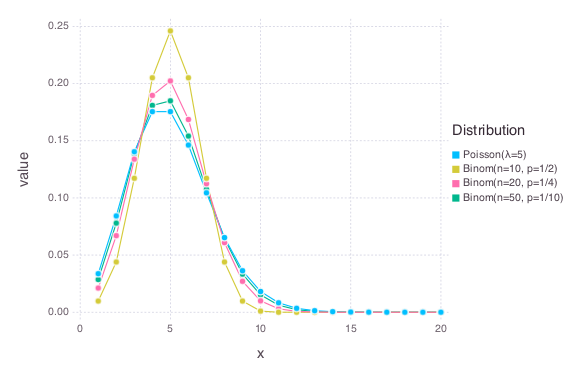
\includegraphics[height=4in,width=6in]{poisson_plot_mult.png}
            \end{solution}
        \end{enumerate}
        \item What distribution does an indicator random variable have?
        \begin{solution}
        It is Bernoulli distributed. An indicator $1_{A}$ has $P(1_{A} = 1) = P(A)$ and $P(1_{A} = 0) = P(\bar{A}) = 1 - P(A)$.

        Part of the appeal of an indicator is that $E[1_{A}] = P(A)$, which is a useful property we'll see later on.
        \end{solution}
        \item Show that for any indicator variable $X$, $E[X] = E[X^2]$.
        \begin{solution}
            $X$ and $X^2$ have the same distribution, actually! $X^2 = X$ in all cases because $X = 0$ or $X = 1$, meaning that they also have the
            same expectation.
        \end{solution}
    \end{enumerate}
    \newpage
        \section{Problems}
        \begin{enumerate}
            \item You roll a six-sided balanced die until you get the first 6. How many dots do you accumulate, on average, including the 6 on the last roll?
            \begin{solution}
                There is a formal way to do this problem. But the intuitive way is to first determine the expected number of rolls to roll a 6. The distribution is $Geom(1/6)$, so we expect
                $6$ rolls. Five of those weren't rolling a six, and the expected value of a roll that isn't a six is $\frac{1+2+3+4+5}{5} = 3$, so we end up with $5 \cdot 3 + 6 = 21$. 

                This is actually the right way to do it, and is formally supported by Wald's identity.
            \end{solution}
            \item \begin{enumerate}
                \item You want to collect 20 Marvel superheroes, which come randomly in cereal boxes. How many cereal boxes do you expect to buy before you collect them all?
                \begin{solution}
                    This is a bunch of geometric distributions in sequence, $X = X_1 + \ldots + X_{20}$, where $X_i \sim Geom(\frac{21 - i}{20})$ represents how many cereal boxes
                    we need to buy before collecting the $i$th superhero, assuming we've already collected $i-1$. This is because there are $20 - (i - 1)$ choices for the next superhero.
                    Then we have $\sum_{i=1}^{20} \frac{21-i}{20}$.
                \end{solution}
                \item Now let's say you can only buy 20 cereal boxes. What's the expected number of superheroes you'll get?
                \begin{solution}
                    Let's write it as a sum of indicators, $X = X_1 + \ldots + X_{20}$. $X_i$ will be 1 if we got the $i$th superhero, and 0 otherwise. The probability that we didn't get the $i$th superhero among 20 boxes is
                    $\left(\frac{19}{20}\right)^{20}$. So $E[X_i] = 1 - \left(\frac{19}{20}\right)^{20}$, so $E[X] = 20 \left(1-  \left(\frac{19}{20}\right)^{20}\right)$.
                \end{solution}
                \end{enumerate}
            \item Let's look at completely random $n$-length binary sequences where $n \geq 2$. We want to count how many `double-ones' we get in the sequence, i.e. the sequence 011101101 has 3 `double-ones'. 
            \begin{enumerate}
                \item What's the expected value of number of double-ones we get for a sequence of length $n$?
                \begin{solution}
                    Write it as sum of indicators. Let $X_i$ be one if position $i$ ends in a double-one. $X_1$ is never 1, but the probability of any other $X_i$ being one is $1/4$, so
                    $E[X] = \sum_{i=2}^n E[X_i] = \frac{n-1}{4} = \mu$.
                \end{solution}
                \item What's the variance?
                \begin{solution}
                    We want to find $var[X] = E[X^2] - \mu^2$. We already know $\mu$, and it's left to find $E[X^2]$. But \[
                        X^2 = (X_2 + \ldots + X_n) (X_2 + \ldots + X_n) = \sum_{i = j} X_i^2 + \sum_{i \neq j} X_i X_j
                    \]
                    This is a common technique we use a lot. By linearity of expectation, we have \[
                        E[X^2] = \sum_{i = j} E[X_i^2] + \sum_{i \neq j} E[X_i X_j] = \sum_{i = j} E[X_i^2] + 2 \cdot \sum_{i < j} E[X_i X_j]
                    \]
                    
                    The second equality comes from the fact that we notice that all pairs $(i, j)$ where $i \neq j$ counts the same pair twice, once where $i < j$
                    and once where $i > j$.
                    We know $E[X_i^2] = E[X_i] = 1/4$, so $\sum_{i = j} E[X_i^2] = \frac{n-1}{4}$.

                    For the $i < j$ case, we need to figure out $E[X_i X_j]$. If $j > i + 1$, we're fine, and the two double-ones are independent. But if $j = i + 1$, then the 2nd double-one
                    has a $1/2$ chance of happening if the first one does! So now we get \[
                        E[X^2] =  \sum_{i = j} E[X_i^2] + 2 \cdot \left(\sum_{i = j - 1} \frac{1}{16} + \sum_{i > j - 1} \frac{1}{8}\right)
                    \]
                    There are $(n-1)^2$ total terms we're looking at, of which $n$ are the first summation, $n-2$ are in the second, and the rest go to the third. The algebra is a little tedious, what's
                    important is understanding why we split up the terms in this way.
                \end{solution}
            \end{enumerate}
    \end{enumerate}
    \end{document}
        